\chapter{System Programming Overview}

The world of software development can be broadly divided into two major domains: \emph{application programming} and \emph{system programming}. When writing an application---be it in Python, Java, or C\#---you implicitly rely on a massive underlying infrastructure. You assume the presence of an interpreter, a virtual machine, and an operating system that seamlessly handles the hardware on your behalf.

Consider what happens when you write a simple script in Python that prints ``Hello, world!''. You execute it, and it works. But \emph{why} does it work? Who provides the Python interpreter? Who handles the fact that the CPU cannot natively understand Python? Who allocates the memory for your variables, interacts with the filesystem, and connects to the network? The answer is an entire hidden software ecosystem: the operating system kernel, device drivers, compilers, linkers, loaders, and runtime libraries.

System programming is the discipline of building that exact infrastructure. It is the software that acts as the intermediary between raw hardware (CPU, memory, peripherals) and high-level applications. As the professor put it: \emph{``The amount of system code involved in allowing even a simple application to run is astonishing.''}

\begin{figure}[h!]
    \centering
    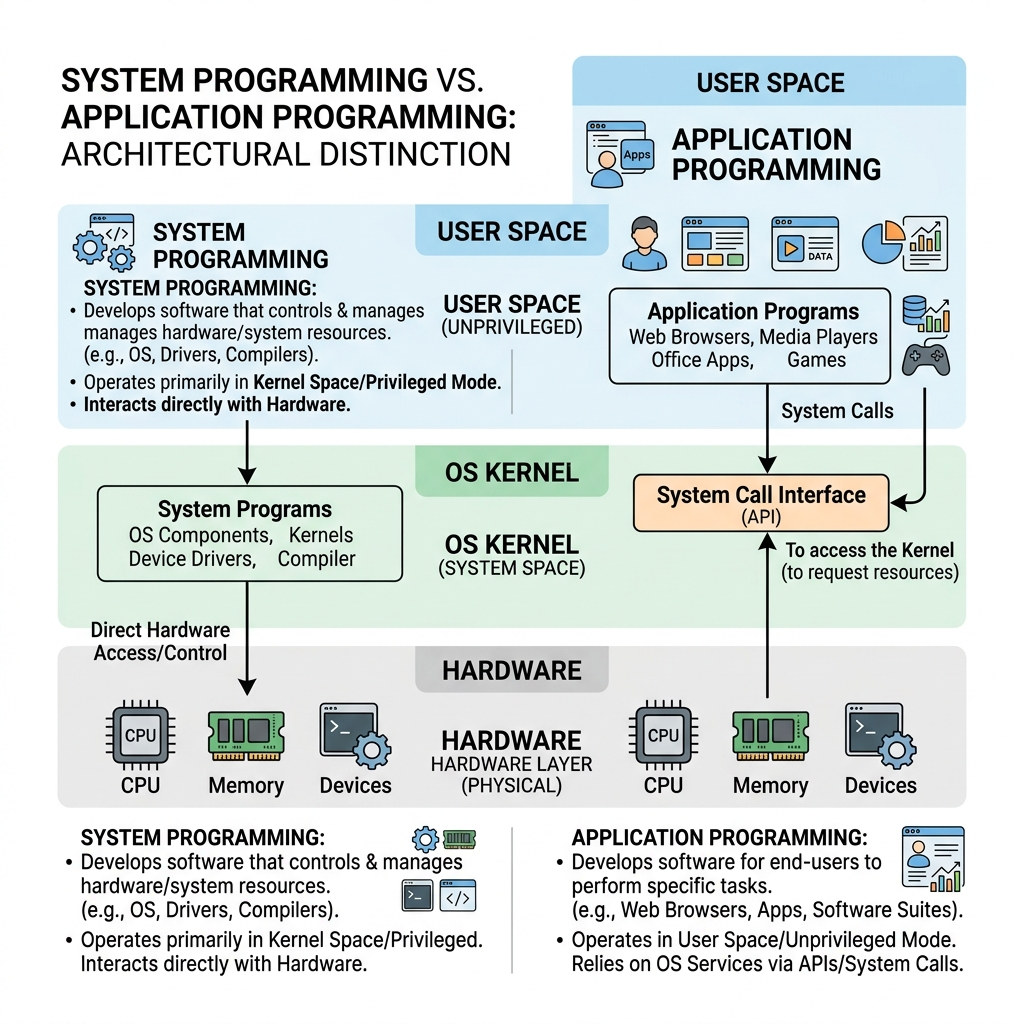
\includegraphics[width=0.8\textwidth]{images/system_architecture.png}
    \caption{The typical software stack, illustrating how system programming bridges the gap between application software and raw hardware.}
    \label{fig:system_architecture}
\end{figure}

% AI-IMAGE-REQUEST: A layered diagram showing Hardware at the bottom, then Kernel/Drivers, then System Software (compilers, linkers, loaders, runtime libs, file systems, DBMS, VMs, crypto), then Application Software at the top. Arrows show the bridging role of system programming.

\section{What is System Programming?}

The scope of system programming is far wider than most students initially imagine. It encompasses every piece of software that must be \emph{particularly efficient}, interact directly with hardware, or provide infrastructure upon which other software depends. Specifically, it includes:

\begin{itemize}
    \item The \textbf{operating system kernel} and all of its internal components;
    \item \textbf{Peripheral drivers}---the code that translates abstract instructions into physical signals for network cards, disks, GPUs, and other hardware;
    \item \textbf{Compilers and interpreters}---the programs that transform source code into something the processor can actually execute;
    \item The \textbf{linker and loader}---tools that ``stitch together'' your code with libraries written by others and load it into RAM when you execute it, without you even noticing;
    \item \textbf{Runtime libraries}---invisible foundations that support every construct of the language you use daily;
    \item \textbf{File systems}, the \textbf{network stack}, \textbf{DBMS engines}, \textbf{virtual machines}, \textbf{cryptographic libraries}, and \textbf{embedded systems firmware}.
\end{itemize}

In short: if a software component must be efficient, interact with hardware, or serve as a foundation for others, it belongs to system programming.

\subsection{The Role of the Runtime Library}

A concept that deserves special attention is the \textbf{runtime library}. High-level programs are not transformed by the compiler into pure machine instructions alone. The compiler also generates calls to a set of support functions---the runtime library---that coordinate the execution environment. Within the runtime library, you find:

\begin{itemize}
    \item \textbf{Completely hidden functions} that are essential for correct operation but invisible to the programmer---for example, functions that check for stack overflow when too many nested calls accumulate;
    \item \textbf{Wrapper functions} that make operating system services accessible---for example, \texttt{fopen()} does nothing more than translate your request into a \emph{system call} that asks the kernel to open a file. The file is managed by the operating system in its kernel; you do not have direct visibility, and the runtime library provides the bridge;
    \item \textbf{Initialization and cleanup code} (the \texttt{\_start}/CRT0 routines discussed later) that prepares the execution environment before \texttt{main()} and tears it down afterward.
\end{itemize}

In essence, the runtime library is the invisible substrate that makes the abstractions of a high-level language actually \emph{work} on real hardware, and it is itself a piece of system software.

\subsection{Resource-Constrained Environments}

A defining characteristic of system programming is operating under \textbf{strict resource constraints}. The professor illustrated this with the example of a home Wi-Fi router: a small device containing a low-cost, low-power CPU, limited RAM, and at least two network interfaces (the ISP-facing one and the local one for your apartment---possibly doubled with Wi-Fi and Ethernet). The software inside that router must guarantee continuous, reliable packet routing, operating within its meager resources.

\begin{insightbox}
\textbf{The Router Example} \\
``If you're building a domestic router, there is a processor inside, there is RAM, there are network interfaces, and there is software. This software must guarantee that the router does its job---routing packets according to the logic you configured---in the context of relatively little RAM. The processor must be cheap so the router can be mass-produced. So we need to avoid waste of memory, CPU cycles, and memory locations. Knowing exactly how many bytes we use and how many CPU cycles we consume \emph{makes sense} in this context.''
\end{insightbox}

In such environments, every byte of memory and every processor cycle counts. You cannot afford expensive abstractions that ``work'' but waste resources. You must know exactly what happens under the hood.

\subsection{Professional Responsibility}

The professor dedicated significant attention to a concept that transcends pure technique: professional responsibility. An engineer is someone who \emph{designs, builds, and deploys systems while assuming responsibility for their correctness and safety}. This is not an abstract concept---it is a concrete, personal commitment.

When asked to define what an engineer is, the core answer is: someone who \textbf{designs, builds, and puts systems into the field}---and \textbf{assumes personal responsibility} for their correct and safe operation. This responsibility rests on two pillars: \emph{theory} (the accumulated knowledge that prevents us from reinventing the wheel or attempting perpetual motion) and \emph{craft} (the practical skill of knowing \emph{how} to use tools effectively and safely, just as soldiers learn to keep the safety on their rifle).

\begin{warningbox}
\textbf{Real-World Responsibility} \\
When you enter an elevator, it says ``maximum capacity: 400 kg.'' Someone signed their name to certify that up to that limit, the elevator is safe. If it breaks and someone is hurt, that engineer is personally accountable. The same principle applies to software: if you write the ABS braking controller for a car, and someone dies because of a bug rooted in your superficiality, you carry that weight. If you write ATM software and a retiree loses their entire pension because of a security flaw, that responsibility is yours.
\end{warningbox}

Every time you sit down, you trust that whoever built the chair designed it to hold your weight. Every time you walk under a video projector mounted on the ceiling, you trust that the person who installed it did so correctly. We all live embedded in a web of trust---and as software engineers, others will trust our code with their safety, their data, and their money.

The professor also referenced the Morandi bridge collapse in Genoa as a stark example: \emph{``The people who left the bridge without performing proper maintenance were murderers. Over 40 people died. Because someone said `Yes, but what do you want? It will hold up.' The same happens to those who write software with superficiality instead of precision.''}

\begin{insightbox}
\textbf{The Web of Trust} \\
``All of us live by trusting that others have built things that are suitable for their context. And others will trust \emph{us} in the same way. What you are doing here---your studies---is very important to focus on well. We are here to become adults in a society that, with all its contradictions and limits, seeks to create a better world. And this goes through assuming responsibilities.''
\end{insightbox}

\subsection{Building Knowledge: The Concept Dependency Chain}

The professor stressed that the topics in this course build \emph{vertically}---each concept depends on the previous ones being solid, unlike courses where concepts are explored horizontally and can be studied in any order.

\begin{insightbox}
\textbf{The Concrete Floors Analogy} \\
``You can't build the roof of a house and then work downward to the foundations. And when you pour a new concrete floor, you must wait 28 days for it to solidify before you can build on top. The same applies to these concepts: if you don't understand how memory is managed, it is useless to talk about ownership. If you don't understand ownership, it is useless to talk about lifetimes. If you don't understand lifetimes, it is useless to talk about concurrency. They build one on top of the other. And they assume that the bottom floor is solid.''
\end{insightbox}

This is why the course is structured to alternate lectures week by week, giving students time to \emph{assimilate}---the professor compared it to eating regularly rather than fasting for a month and then gorging: \emph{``Study must be dosed so you can actually digest it. Cramming the night before an exam is like stuffing yourself after a month of fasting---you'll just vomit it all back up.''}

\section{Language Selection: Why Not Java, Python, or Go?}

To write high-performance system software, you need a language that gives you total control over how memory, CPU, and I/O are used. This criterion immediately disqualifies languages with automatic \textbf{Garbage Collection (GC)}: Java, JavaScript, Python, C\#, Go, and similar languages.

\subsection{The Garbage Collection Problem}

Languages with garbage collection work on a simple principle: you request memory when you need it, but when you no longer need it, you simply \emph{abandon it}. At some point, a garbage collection cycle will reclaim the abandoned memory and make it available again. This convenience comes at a steep price.

\begin{insightbox}
\textbf{The Washing Dishes Analogy} \\
``Languages with a garbage collector are like someone who never washes dishes after a meal. You eat lunch, leave the dish in the sink. You do it for one day, two, three, four, five. When the pile is high, you decide to wash them all at once. It works---somehow---besides the fact that bacteria proliferate. But the problem is that you need an enormous number of dishes! If you work in a resource-constrained context, you must wash the dishes \emph{every time}---which means releasing memory explicitly.''
\end{insightbox}

The global memory footprint of a garbage-collected application is always significantly larger than the strictly necessary minimum, because memory is released in ``waves'' rather than immediately when no longer needed.

\subsubsection{Stop-the-World, Mark \& Sweep, Reference Counting}

To determine which blocks of memory can be freed, the Garbage Collector must ``stop the world''---\textbf{suspending the entire program's execution} (freezing all threads) to examine the heap in a static snapshot. Starting from all variables on the stack and in global variables, it recursively traverses all pointers. Everything not reachable from this root set can be freed. This is the essence of the \textbf{Mark \& Sweep} family of algorithms, the most famous GC approach. An alternative approach is \textbf{Reference Counting}, which tracks how many references point to each object.

The ``stop-the-world'' pause is \textbf{non-deterministic}---it can last from milliseconds to entire seconds, depending on how much heap must be analyzed. The professor made this vivid: \emph{``In one second, your CPU performs about a billion operations. If the CPU's clock cycles were heartbeats, a billion heartbeats would be centuries. That's how expensive a GC pause can be.''}

In a real-time system---a laser cutter, a car's ABS brake controller, or an industrial press---such pauses are completely unacceptable. You cannot stop controlling the laser for a millisecond to do garbage collection.

\subsection{The Remaining Candidates}

With GC-based languages excluded, few options remain for system programming:
\begin{itemize}
    \item \textbf{C}---the historic ``battle horse'' on which operating systems and most legacy system software were built;
    \item \textbf{C++}---offering a higher level of abstraction than C, with more structured programming capabilities;
    \item \textbf{Rust}---the modern contender, designed to solve C/C++'s safety problems;
    \item \textbf{ZIG} and \textbf{Carbon}---niche languages without significant adoption yet;
    \item \textbf{Swift}---relevant primarily in the Apple ecosystem, with an uncertain broader future.
\end{itemize}

\subsection{Why This Course Uses Rust}

Rust is not simply ``another system language.'' It was designed to solve a specific class of problems that have plagued C and C++ for decades, by encoding memory management responsibilities directly into the type system.

\begin{insightbox}
\textbf{The Mental Model Quote} \\
``Rust forces us to mature a coherent mental model of how things actually work. Once we understand it, whether we then write in Rust, Python, or Java, it doesn't matter anymore---because the underlying principles are clear to us. Rust is like Italian in this lecture: it shapes how we \emph{think} about the problems, not just how we express solutions.''
\end{insightbox}

The critical point is that \textbf{Rust's compiler refuses to compile code that violates memory safety rules}. In C, the compiler says ``ok'' and your program---with its bug---goes into execution, maybe apparently works, and then crashes in production at 3 AM. In Rust, the error surfaces at compile time, when it is still cheap to fix.

\begin{insightbox}
\textbf{The Drunk Driving Analogy} \\
``The difference between catching a bug at compile time versus at runtime is like being caught drunk \emph{before} causing an accident versus being discovered the day after you've killed someone because you couldn't brake in time. A compile-time error is infinitely more valuable than a runtime crash.''
\end{insightbox}

Rust is not an absolute guarantee---it cannot detect infinite loops or deadlocks in general---but it eliminates the vast majority of memory-related bugs that cause catastrophic damage in C programs. The professor emphasized: \emph{``In C, the program compiles---but that doesn't mean it works. If you've tried building a linked list in C, you know the enormous gap between `it compiles' and `it actually works.' Segmentation faults tell you that story.''}

\section{Executable Programs and Their Execution}

To take responsibility for how software behaves, we must deeply understand how hardware executes it.

\subsection{What Is an Executable Program?}

An executable program is, at its essence, a \textbf{sequence of binary numbers}. It contains machine instructions, data values, configuration information, and control structures. Understanding this representation is crucial:

\begin{itemize}
    \item The \textbf{meaning of machine instructions} is hardwired into the specific processor's hardware. An opcode like \texttt{7B5F} on an x86 processor means one precise thing; on an ARM processor, the same bit pattern might mean something completely different or be entirely invalid. Programs are therefore \emph{architecture-specific}---compiled for a particular processor family.
    \item The \textbf{meaning of other data} (constants, configuration structures, OS-specific sections) depends partly on the instruction semantics (e.g., the byte following a ``load immediate'' instruction is the value to load) and partly on the operating system that will load and execute the program.
\end{itemize}

\subsection{The Loader: From Disk to Execution}

How a program gets into memory depends on the type of system.

\textbf{Embedded systems (e.g., Arduino):} The compiled program is transferred directly into the microcontroller's flash memory via a hardware programmer (USB-serial connection). When the device resets, the processor begins executing from a predefined address. There is no file system, no operating system---the program runs on bare metal. Importantly, an Arduino \textbf{has no MMU}---it is too simple internally---so the addresses your program uses are the physical addresses directly.

\textbf{General-purpose systems (PC, server, smartphone):} Programs reside as files on disk. To execute them, the operating system uses a component called the \textbf{loader}:
\begin{enumerate}
    \item It reads the executable file (\texttt{.exe} on Windows, an \textbf{ELF} file on Linux);
    \item It identifies which \textbf{dynamic libraries} the executable depends on (\textbf{DLL} on Windows, \textbf{.so} on Linux) and loads them as well;
    \item It transfers all necessary code and data from disk to RAM;
    \item It configures internal structures and \textbf{creates a process with a thread} dedicated to executing instructions sequentially.
\end{enumerate}

The operating system then schedules this thread, letting it execute for a time slice (a few milliseconds), then freezing it and letting other programs run. This is how your PC can have 27 open programs, each seemingly running simultaneously.

\subsection{The Fetch-Decode-Execute Cycle}

Once the program is in RAM, the CPU operates on a continuous, elementary cycle:

\begin{enumerate}
    \item \textbf{Fetch}: The CPU reads the next instruction from RAM at the address stored in a dedicated register called the \textbf{Program Counter} (or \textbf{Instruction Pointer} on x86). This register always points to the next instruction to execute.
    \item \textbf{Decode}: The fetched instruction is analyzed internally. The CPU determines what kind of operation it is: an addition, a multiplication, a data transfer, a jump, etc.
    \item \textbf{Execute}: The hardware activates the necessary logical units to perform the operation. Effects may include updating internal registers, setting flags, writing to memory, or activating I/O lines that command external electronics.
\end{enumerate}

Modern processors operate in \textbf{pipeline}: while executing one instruction, they simultaneously decode the next and fetch the one after that. This allows CPUs to be particularly efficient. But conceptually, the model remains this simple cycle: \emph{Fetch-Decode-Execute, Fetch-Decode-Execute}, endlessly.

\section{The Address Space and the MMU}

\subsection{Memory as an Enormous Array}

From a program's perspective, memory can be imagined as a \textbf{huge array of bytes}, each identified by a numerical index called an \emph{address}. The CPU can read or write individual bytes or groups of 2, 4, or 8 bytes at a time, depending on the data width.

The maximum number of theoretically addressable cells depends on the processor architecture. A 64-bit CPU like Intel x64 would nominally have $2^{64}$ addresses---an astronomical number. However, for practical implementation reasons, the \textbf{effective address space is limited to $2^{48}$} cells (approximately 281 terabytes). Obviously, your PC does not have that much physical RAM.

\begin{memoryblock}
\textbf{Address Space Sizes} \\
\begin{itemize}
    \item A 32-bit processor has indices from $0$ to $2^{32}-1$, giving approximately \textbf{4 GB} of addressable space.
    \item A 64-bit processor nominally has $2^{64}$ addresses, but current implementations use only \textbf{48 address lines}, yielding $2^{48} \approx$ \textbf{281 TB} of virtual address space.
    \item Your actual physical RAM (e.g., 16 GB) is a tiny fraction of this virtual space.
\end{itemize}
\end{memoryblock}

This leads to a critical distinction:
\begin{itemize}
    \item The number of \textbf{potentially addressable cells} depends on the processor architecture;
    \item The number of \textbf{actually usable cells} is limited by the installed physical RAM and controlled by the operating system.
\end{itemize}

Consequently, a program's address space is not a uniform, contiguous block---it is a \textbf{sparse space}, where only certain zones are mapped and accessible.

\subsection{Virtual vs. Physical Addresses: The MMU}

The addresses your program uses are \textbf{not} the actual physical hardware addresses of the RAM chips. They are \textbf{virtual addresses}. The CPU's hardware \textbf{Memory Management Unit (MMU)} translates these virtual addresses into physical addresses on the fly, using a \textbf{per-process translation table} maintained by the operating system.

This is not a universal feature: if you have an Arduino, there is no MMU---it is too simple internally---and the addresses you use are the physical addresses directly. But on any modern PC, server, or smartphone, the MMU is always present.

\begin{insightbox}
\textbf{The Parking Zones Analogy} \\
``The operating system manages memory zones just like parking zones in a city. White stripes mean you can park freely. Blue stripes mean you must pay. Yellow stripes are reserved. The operating system marks each memory zone with permissions: this zone can be read but not written; this zone can be read and executed; this zone is completely off-limits. These `stripes' tell the hardware what operations are allowed.''
\end{insightbox}

The MMU provides three crucial benefits:

\textbf{1. Isolation between processes:} If two programs---say, Notepad and your application---both use virtual address \texttt{0x7F799000}, the MMU maps each to a \emph{different} physical location. They cannot interfere with each other's memory. Without this mechanism, two programs would constantly corrupt each other.

\textbf{2. Permission control:} The MMU, directed by the OS, can mark each memory page as readable, writable, and/or executable, independently. The executable code segment is typically marked read+execute but not write---any attempt to modify running code triggers an immediate error.

\textbf{3. Virtual memory exceeding physical:} The OS can make a program \emph{believe} it has access to more memory than physically exists. If you have 16 GB of RAM and request 20 GB, the OS grants it. It maps the 16 GB to physical RAM and marks the rest as ``not currently backed.'' When you access an unbacked page, the OS intervenes, finds physical RAM (possibly by saving another program's unused page to disk---the \emph{swap} or \emph{page file}), updates the translation table, and lets you proceed. This is entirely transparent to your program.

\subsection{Practical Effects: Segfault, Page Fault, and Thrashing}

Normally, all this machinery is invisible. But three situations make it painfully visible:

\textbf{Segmentation Fault:} When a program accesses a virtual address that is \emph{not mapped} in its address space, or that is mapped with insufficient permissions, the MMU generates a hardware interrupt. The OS intercepts it and brutally terminates the process. The ``Segmentation fault'' message you have surely seen in C programs is precisely this.

\textbf{Page Fault:} When a program accesses a virtual address that is mapped but whose physical backing has been temporarily saved to disk. The MMU generates an interrupt, the OS loads the data from disk back into RAM, updates the translation table, and resumes execution. It is transparent to the program---but enormously expensive:

\begin{memoryblock}
\textbf{Page Fault Cost Analysis} \\
A normal RAM access costs approximately \textbf{28 nanoseconds}. A page fault can elevate this to \textbf{3 milliseconds}---about \textbf{100,000 times slower} (the professor says ``50,000 times,'' but the order of magnitude is the key point). Once the 4K page is loaded, subsequent accesses within that page are fast again until the next page fault occurs.
\end{memoryblock}

\textbf{Thrashing:} The extreme case where the system has so many simultaneous memory demands that it spends more time swapping pages between RAM and disk than actually executing programs. The machine practically freezes---you can hear the disk growling, but nothing progresses. The professor's advice: \emph{``In that situation, the only cure is usually to kill everything and start over.''}

\section{Memory Hierarchy and Cache}

\subsection{Why the CPU Does Not Access RAM Directly}

Between the CPU and RAM sits the \textbf{cache}---a small but incredibly fast memory hierarchy (L1, L2, L3). This exists because there is an enormous speed discrepancy: the CPU is thousands of times faster than RAM. If the CPU had to wait for RAM on every access, it would waste almost all its time waiting.

The cache exploits the \textbf{principle of locality}: if a program has just accessed address $I$, it is very likely to access $I+1$, $I+2$, $I+3$ soon (spatial locality), or address $I$ again (temporal locality). When the cache reads address $I$, it pre-fetches an entire block of adjacent addresses, keeping them ready for subsequent accesses.

\begin{insightbox}
\textbf{The Supermarket Analogy} \\
``When you go to the supermarket, you don't buy one bottle of water at a time. You buy a whole case, bring it home, and take bottles one by one from the pantry. When the case is empty, you go back to the supermarket. The CPU cache works exactly the same way: it fetches a whole block of data and keeps it close, so the next accesses are almost free.''
\end{insightbox}

\subsection{Impact on Data Structure Choices}

This principle has concrete consequences for data structure selection. A \texttt{Vec<T>} (Rust's dynamic array, equivalent to Java's \texttt{ArrayList}) stores elements in \textbf{contiguous memory positions}. When you access element 0, the cache automatically loads elements 1, 2, 3, ..., $N$ nearby. Subsequent iterations find data already in cache: extremely fast.

A \texttt{LinkedList<T>}, by contrast, stores each node at an \textbf{arbitrary location in the heap}. The next node can be hundreds or thousands of addresses away. Each traversal step potentially causes a \textbf{cache miss}---the cache must fetch new data from RAM, costing vastly more time.

\begin{figure}[!ht]
    \centering
    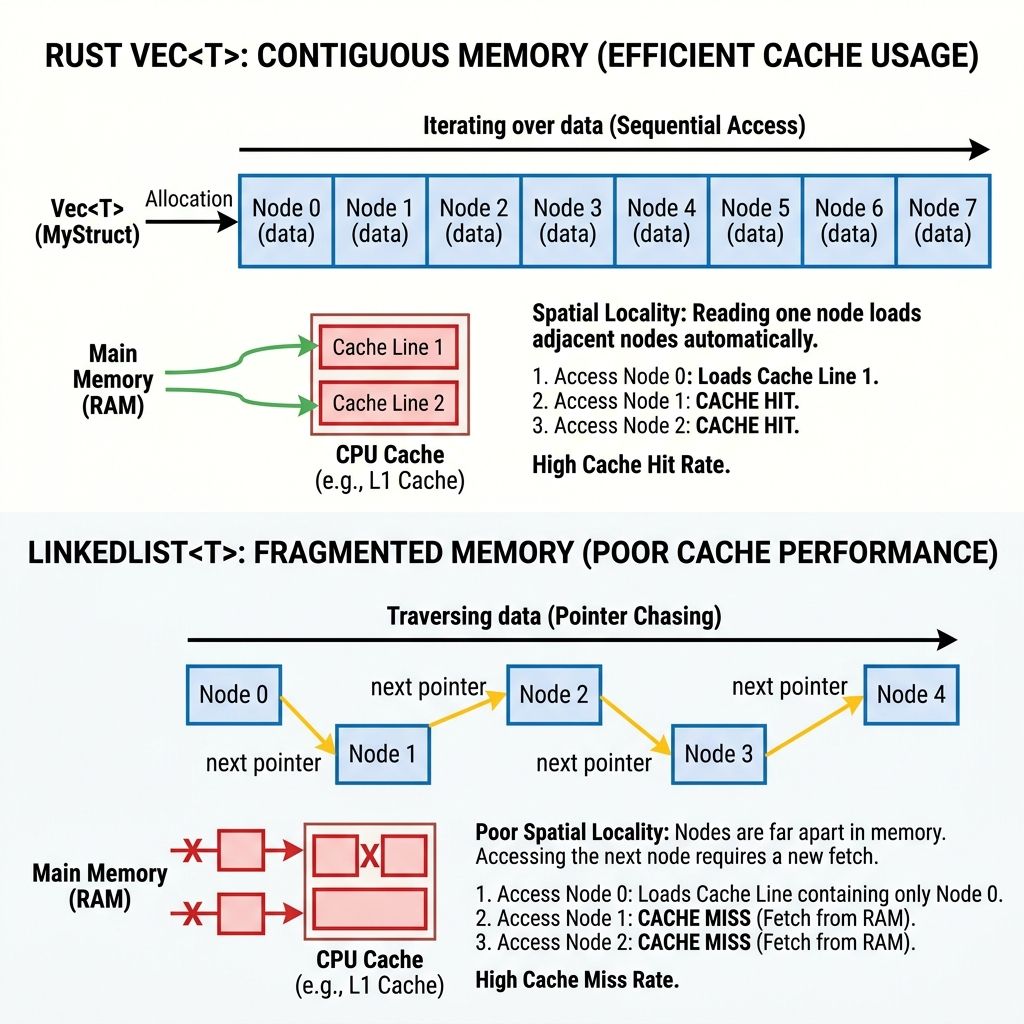
\includegraphics[width=\textwidth]{images/cache_locality.png}
    \caption{Visualizing how Contiguous Memory (Vec) maximizes CPU Cache efficiency compared to Fragmented Memory (LinkedList).}
\end{figure}

The professor used another vivid image: \emph{``With a LinkedList, it's like having a glass of cold water, then wanting a natural one---back to the supermarket! Then you want a Coke---back again! You accomplish very little. The LinkedList benefits very little from the cache.''}

The linked list does have algorithmic advantages (O(1) insertion/removal with node access), but awareness of the cache cost is essential: in practice, \texttt{Vec<T>} is often faster even for operations where the linked list has better theoretical complexity.

\section{The Execution Model: What the Language ``Pretends''}

The C/C++ (and Rust) execution model makes several simplifying assumptions that do not correspond to physical reality but allow the programmer to reason more easily:

\begin{enumerate}
    \item The program is the \textbf{sole user} of the computer (the only evidence of other programs comes from shared resources like the file system);
    \item It can access \textbf{any cell} in the address space (a pointer is a number valid from zero to the maximum integer);
    \item Execution is \textbf{sequential}---one instruction after another, with no inherent parallelism;
    \item There are \textbf{no limits} to the number of instructions, time, or memory available.
\end{enumerate}

Obviously these assumptions are all false---limits exist and condition how programs must be written---but the compiler and OS work together to make them true \emph{to the extent possible}. When reality exceeds the illusion (memory exhaustion, stack overflow, illegal access), the illusion shatters and errors appear.

The professor elaborated on each failure mode: memory is not infinite---as much as the operating system can make the virtual space appear larger than physical RAM, even the disk eventually fills up. The stack has a finite depth, so purely recursive programs may be infeasible (the stack overflow). And even though modern processors have 4 or 8 cores capable of true parallelism, the C/C++ execution model does not inherently expose this---concurrency must be explicitly programmed.

\subsection{The Entry Point: \texttt{main(argc, argv)} and the Hidden Startup}

Every C/C++ program has a well-defined entry point: the function \texttt{main()}, which accepts two parameters:

\begin{lstlisting}[language=C]
int main(int argc, char* argv[])
\end{lstlisting}

\texttt{argc} is an integer indicating the number of command-line arguments. \texttt{argv} is an array of pointers to strings (the arguments themselves), terminated by a null pointer. This is the \emph{first convention} of the C language: computation starts here.

But \texttt{main()} is \textbf{not the true starting point}. Before \texttt{main()}, the \textbf{runtime library} executes hidden initialization code---often called \texttt{\_start} or \texttt{CRT0} (C Runtime Zero)---that sets up the stack, initializes global variables, prepares the heap allocator, and performs other housekeeping. After \texttt{main()} returns, additional cleanup code runs. The programmer never sees this, but it is always there.

Within the execution flow, two fundamental data structures manage memory:
\begin{itemize}
    \item The \textbf{Stack}---for local variables, function parameters, return addresses, and the history of function calls;
    \item The \textbf{Heap}---for dynamically allocated memory whose lifetime is not tied to any single function.
\end{itemize}

In C++, there is an additional element: the stack also carries data needed for \textbf{structured exception handling}---the mechanism for handling situations where computation cannot proceed (disk broken, network down, disk full). In JavaScript/TypeScript, there would also be a \textbf{message queue} for event handling---the structure that allows the program to receive mouse clicks, timer events, network data arrivals, and other asynchronous notifications.

\begin{warningbox}
\textbf{The Processor Does Not Know About Stack or Heap} \\
It is important to understand that the \emph{processor itself} is entirely unaware of the stack and heap as concepts. From the CPU's perspective, they are simply memory addresses like any other---it reads and writes wherever it is told to. The stack and heap are abstractions maintained by the compiler, the runtime library, and the operating system, not by the hardware. The CPU has no knowledge of whether it is reading a local variable from the stack or a dynamically allocated block from the heap---it only sees addresses.
\end{warningbox}

\section{The Stack}

\subsection{Structure and Properties}

The Stack is an automatically managed block of memory, typically around \textbf{1 MB} in size, allocated when the program starts. It operates on a \textbf{Last-In, First-Out (LIFO)} basis---like a pile of plates. When a function is called, a new frame is pushed onto the top; when it returns, the frame is popped off.

The stack stores:
\begin{itemize}
    \item \textbf{Local variables} declared within functions;
    \item \textbf{Parameters} passed to function calls (copied by value);
    \item \textbf{Return values} (space reserved by the caller);
    \item \textbf{Return addresses} (where to resume after the function completes);
    \item In C++: \textbf{exception handling data} for structured exception management.
\end{itemize}

The professor summarized its key properties: \emph{``Automatic, extremely fast, deterministic lifetime.''} The stack supports the principle of locality very well, and its management is handled entirely by the compiler-generated code---the programmer does not need to write a single line to manage it.

\subsection{Step-by-Step Code Walkthrough}

\begin{figure}[!ht]
    \centering
    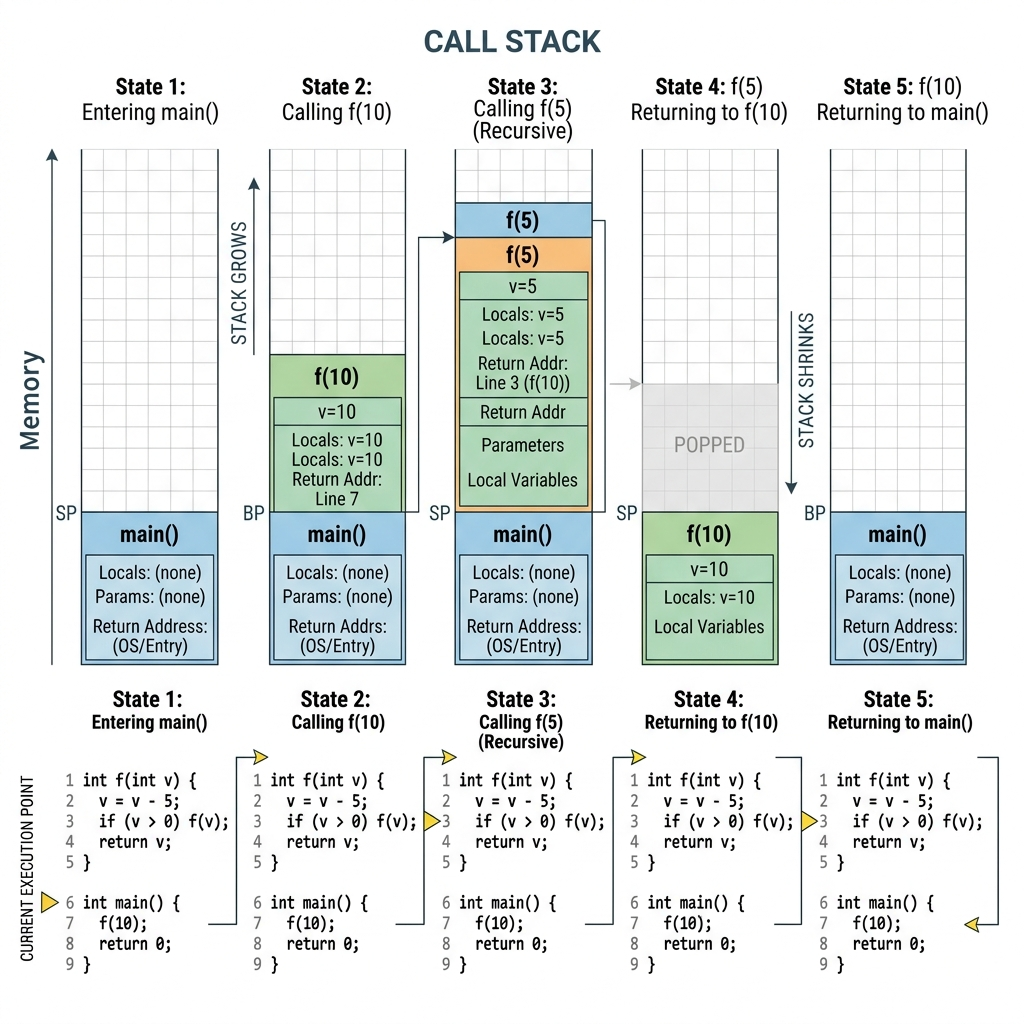
\includegraphics[width=\textwidth]{images/stack_execution.png}
    \caption{Step-by-step anatomy of function calls pushing and popping frames on the Stack.}
\end{figure}

Let us trace exactly what happens in the stack with this C program:

\begin{lstlisting}[language=C]
int f(int a) {
    int i = 5;
    if (a > 0) { return a + i; }
    else { return a - 1; }
}

int main() {
    int v = 9;
    v = f(v);
    return 0;
}
\end{lstlisting}

\textbf{Step 1 --- Startup:} Before \texttt{main()} even begins, the hidden \texttt{\_start}/CRT0 code runs. It initializes the stack and reserves space for the return value of \texttt{main()} (the ``\texttt{...}'' or ``res'' slot).

\textbf{Step 2 --- \texttt{int v = 9}:} The stack grows by 4 bytes. The value \texttt{9} is written into this new space. The local variable \texttt{v} now exists on the stack.

\textbf{Step 3 --- Preparing the call \texttt{f(v)}:} Before jumping to function \texttt{f}, the caller prepares the stack:
\begin{enumerate}
    \item Space is reserved for \texttt{f}'s return value (another ``\texttt{...}'' slot);
    \item The \emph{value} of \texttt{v} is \textbf{copied} as parameter \texttt{a}---note: this is a \emph{copy}, not a reference; \texttt{a} is completely independent of \texttt{v};
    \item The \textbf{return address} is pushed---the address of the instruction in \texttt{main()} where execution should resume after \texttt{f} completes (the assignment \texttt{v = ...}).
\end{enumerate}

\textbf{Step 4 --- Inside \texttt{f()}:} The function begins executing. It declares \texttt{int i = 5}---the stack grows further to hold this local variable. At this point, the stack contains: main's res, \texttt{v}=9, f's res, \texttt{a}=9, return address, \texttt{i}=5.

\textbf{Step 5 --- \texttt{return a + i}:} Since \texttt{a} is 9 and \texttt{i} is 5, the result is \texttt{14}. This value is written into the reserved return-value slot. Then \texttt{f}'s local variables (\texttt{i}) and parameters (\texttt{a}) are invalidated as the stack contracts. The Program Counter jumps to the saved return address.

\textbf{Step 6 --- Back in \texttt{main()}:} The value \texttt{14} is read from \texttt{f}'s return slot and assigned to \texttt{v}. Now \texttt{v = 14}. All traces of \texttt{f}'s execution on the stack have been erased.

\textbf{Step 7 --- \texttt{return 0}:} The value \texttt{0} is written into \texttt{main}'s return-value slot. The stack contracts further. Execution returns to the hidden startup library (\texttt{\_start}/CRT0), which performs final cleanup before terminating the process.

\begin{insightbox}
\textbf{The AirBnb Analogy} \\
``The stack's memory is like an AirBnb apartment. You check in, stay three days, use it for your vacation, then check out and leave. The apartment is not demolished---it stays there, ready for the next guest. If after calling \texttt{f()} you call \texttt{g()}, function \texttt{g} will reuse the exact same memory that \texttt{f} just used for its own calculations. It's always the same memory, used and regularly recycled.''
\end{insightbox}

\subsection{The Two Constraints of the Stack}

This enormous efficiency comes with two fundamental constraints:

\textbf{Temporal Constraint:} Data on the stack \emph{cannot last longer than the function (or block) in which it was declared}. When the function returns, the stack pointer moves back down and that memory is logically gone. You \textbf{cannot return a pointer to a local variable}---it will become a dangling pointer the instant the function exits.

\textbf{Dimensional Constraint:} The stack has a finite size (typically $\sim$1 MB). You cannot use it for large data or data whose size is unknown at compile time. Even without massive data, this limits \textbf{recursion depth}: a recursive factorial implementation makes the stack grow with each recursive call. At some point, the stack hits its limit---a \textbf{stack overflow}---even though the computation has not finished.

The professor noted: \emph{``Since the stack starts at 1 megabyte, after putting a single very large local variable, there might be no room for anything else. That's why we need the heap.''}

\section{The Heap}

\subsection{Why the Stack Is Not Enough: Three Reasons}

There are three situations where the stack is insufficient:
\begin{enumerate}
    \item \textbf{The data must outlive the function that created it}---for example, you allocate a buffer inside a function and want to use it from another;
    \item \textbf{The data's size is unknown at compile time}---for example, an array whose size depends on user input;
    \item \textbf{The data is too large} for the stack---a 10 MB image cannot live in a stack frame.
\end{enumerate}

For these cases, the \textbf{Heap} (also called \emph{Free Store} in C++) exists: a much larger memory area where blocks can be allocated and released dynamically, with lifetimes not tied to any specific function.

\subsection{The Key Difference from the Stack}

On the stack, declaring \texttt{int i = 5;} is sufficient: the compiler knows exactly where \texttt{i} will go (relative to the stack pointer), and the generated machine code handles everything automatically.

On the heap, there is no such automatism. You must:
\begin{enumerate}
    \item \textbf{Explicitly request} a block of memory using a dedicated function (\texttt{malloc} in C, \texttt{new} in C++);
    \item \textbf{Receive a pointer} to the beginning of the allocated block---this is the \emph{only} way to access it;
    \item \textbf{Use the block} through that pointer (using the dereference operator \texttt{*});
    \item \textbf{Explicitly release} the block when you no longer need it, using the dual function (\texttt{free} in C, \texttt{delete} in C++).
\end{enumerate}

\subsection{Step-by-Step C++ Code Walkthrough}

Let us trace a heap allocation example:

\begin{lstlisting}[language=C]
int* f(int a) {
    if (a > 0) {
        return new int[a];  // allocate an array of 'a' ints on the heap
    } else {
        return nullptr;
    }
}

int main() {
    int v = 2;
    int* buffer = f(v);   // buffer points to the heap block
    // ... use buffer ...
    delete[] buffer;       // explicitly release
    buffer = nullptr;      // discipline: prevent dangling pointer
    return 0;
}
\end{lstlisting}

\textbf{\texttt{int v = 2}:} A local variable on the stack. Normal.

\textbf{\texttt{int* buffer = f(v)}:} The variable \texttt{buffer} is a \textbf{pointer}---it occupies 8 bytes on the stack (on 64-bit systems), but its value (an address) is not yet initialized (the ``three dots''). Then \texttt{f} is called.

\textbf{Inside \texttt{f()}:} The function receives \texttt{a = 2}, verifies it is positive, and executes \texttt{new int[2]}. If this had been C, we would write \texttt{malloc(2 * sizeof(int))}. The \texttt{new int[a]} tells the runtime: ``prepare a contiguous space of as many integers as the value in variable \texttt{a}.'' The runtime finds space somewhere in the heap---it is irrelevant whether it is a bit lower or higher---marks it as occupied, and returns a pointer to the first byte.

\textbf{The function returns the pointer:} The stack frame of \texttt{f} is dismantled, but the heap block \textbf{remains intact}---it does not belong to any stack frame. The variable \texttt{buffer} in \texttt{main} receives this address.

\textbf{\texttt{delete[] buffer}:} This is the act of \emph{restitution}. It informs the runtime that the block is no longer needed. The runtime marks it as available for future allocations. \textbf{But the pointer \texttt{buffer} still contains the old address!} That block no longer belongs to the program, but the pointer doesn't know that.

\textbf{\texttt{buffer = nullptr}:} This is the disciplined programmer's safety measure. By explicitly setting the pointer to null after deletion, any future accidental access generates a controlled segfault instead of silently corrupting memory. \emph{The language does not force you to do this}---you must have the discipline to do it yourself.

\begin{warningbox}
\textbf{The \texttt{delete[]} Danger} \\
After \texttt{delete[] buffer}, the pointer \texttt{buffer} still holds the old address. It has become a \emph{dangling pointer}. The owner (the runtime/OS) is now free to give that memory to someone else, or even ``demolish the building.'' Accessing \texttt{*buffer} after deletion is \textbf{Undefined Behavior}. Always set pointers to \texttt{nullptr} after freeing.
\end{warningbox}

\section{Allocation and Deallocation Functions}

\subsection{In C}

The C standard library provides three allocation functions:

\begin{itemize}
    \item \texttt{void* \textbf{malloc}(size\_t s)} --- allocates \texttt{s} bytes, \emph{without initializing them}. Contents are whatever was previously in that memory. Returns \texttt{NULL} on failure.
    \item \texttt{void* \textbf{calloc}(int n, size\_t s)} --- allocates \texttt{n * s} bytes, initializing them all to zero. Safer but slightly slower.
    \item \texttt{void* \textbf{realloc}(void* p, size\_t s)} --- resizes a previously allocated block. If it succeeds, the first portion retains the old data; additional space contains garbage. It might move the block to a new location (the old pointer becomes invalid). Returns \texttt{NULL} on failure (original block remains intact).
\end{itemize}

Deallocation: \texttt{void \textbf{free}(void* p)}.

\subsection{In C++}

C++ adds the keywords \texttt{new} and \texttt{delete}:

\begin{itemize}
    \item \texttt{\textbf{new} T\{args\}} --- allocates memory and calls the constructor;
    \item \texttt{\textbf{new} T[n]} --- allocates an array of \texttt{n} elements;
    \item \texttt{\textbf{delete} p} --- calls the destructor and deallocates;
    \item \texttt{\textbf{delete[]} p} --- calls destructors for all elements and deallocates.
\end{itemize}

\begin{warningbox}
\textbf{Fundamental Rule: Dual Functions} \\
Every block must be released with the \emph{dual} of the function that allocated it: \texttt{malloc} $\leftrightarrow$ \texttt{free}, \texttt{new} $\leftrightarrow$ \texttt{delete}, \texttt{new[]} $\leftrightarrow$ \texttt{delete[]}. Mixing these pairs corrupts the runtime's internal data structures and produces unpredictable behavior.
\end{warningbox}

\section{Address Space Layout}

When a program executes, its virtual address space is divided into distinct zones, each with specific purposes and permissions:

% AI-IMAGE-REQUEST: A vertical diagram of a process's address space showing (from bottom to top or top to bottom): Text segment (read+execute), Read-only data (constants/string literals), Global variables (read+write), Heap (growing upward), free space, Stack (growing downward), and Runtime libraries (DLL/.so). Label each zone with permissions (r/w/x).

\begin{itemize}
    \item \textbf{Executable Code (Text Segment):} Contains the processor's machine instructions. Mapped as \emph{read + execute only}---not writable. Any attempt to modify running code triggers a segfault.
    \item \textbf{Constants (Read-only Data):} Contains string literals (e.g., the \texttt{"Hello world"} in a \texttt{printf} call), global constants, etc. Mapped as \emph{read-only}. Attempting to write here causes a segfault.
    \item \textbf{Global Variables (Data Segment):} Contains variables declared outside any function. Readable and writable. Initialized by the loader \emph{before} \texttt{main()} is called.
    \item \textbf{Stack:} Grows from high addresses downward (on many architectures). Contains function frames with parameters, local variables, and return addresses.
    \item \textbf{Heap:} Grows from low addresses upward. Contains dynamically allocated blocks, managed by the allocator (part of the runtime library).
    \item \textbf{Runtime Libraries:} Memory segments mapped from dynamic libraries (DLL / \texttt{.so}) used by the program.
\end{itemize}

\subsection{Inspecting with \texttt{/proc/<pid>/maps}}

On Linux (or WSL2 on Windows), you can directly observe your program's address space. For any running process with PID \texttt{<pid>}, the file \texttt{/proc/<pid>/maps} (a pseudo-file generated dynamically by the kernel each time you read it) shows every mapped zone with its addresses, permissions, and origin.

\begin{lstlisting}[language=bash]
$ cat /proc/4742/maps
00400000-00452000 r-xp  /usr/bin/myprogram    # executable code
00652000-00653000 r--p  /usr/bin/myprogram    # read-only data
00653000-00654000 rw-p  /usr/bin/myprogram    # global variables
01a3e000-01a5f000 rw-p  [heap]               # heap
7f8a1c000000-...  r-xp  /lib/x86_64.../libc.so.6  # shared library
7ffd4bc9e000-...  rw-p  [stack]              # stack
\end{lstlisting}

You will clearly see that of all $2^{48}$ potential addresses, only tiny fragments are actually mapped. The numbers will differ each time---the OS randomizes locations for security through a mechanism called \textbf{ASLR} (Address Space Layout Randomization)---but the structure is always the same. \textbf{Any attempt to access addresses outside these ranges causes a segmentation fault.}

\section{Variable Lifecycle: Global, Local, Dynamic}

The C/C++ execution model distinguishes three categories of variables, each with fundamentally different properties:

\begin{center}
\begin{tabular}{|l|c|c|c|c|}
\hline
\textbf{Property} & \textbf{Global} & \textbf{Local} & \textbf{Dynamic} \\
\hline
\textbf{Location} & Data segment & Stack & Heap \\
\hline
\textbf{Address} & Fixed (compile/link time) & Relative to stack top & Absolute (runtime) \\
\hline
\textbf{Lifetime} & Entire program & Block/function scope & Until explicit release \\
\hline
\textbf{Initial value} & Loader-initialized & \textbf{Random garbage} & Uninitialized (C) / Constructed (C++) \\
\hline
\textbf{Access} & By name, anywhere & By name, in scope & \textbf{Only via pointer} \\
\hline
\end{tabular}
\end{center}

\textbf{Global variables} have a fixed address determined by the compiler and linker. They exist from program start to program end. If initialized (e.g., \texttt{int x = 27;}), the loader ``paints'' that value into memory \emph{before} \texttt{main()} is called---it is not an executed instruction; the data is pre-loaded.

\textbf{Local variables} exist on the stack, at addresses relative to the current stack top. The compiler cannot say where variable \texttt{i} will be in absolute terms---it only knows at runtime. Their lifetime is tied to the block in which they are declared: they start to exist when execution enters the block, and cease to exist when execution exits it (even if the block is a \texttt{for} loop or an \texttt{if} body, not just an entire function).

\begin{insightbox}
\textbf{Random Garbage in Local Variables} \\
``What do you find when you enter an AirBnb apartment? The mess the previous guest left behind. If the previous guest was clean, great. If not, you're in trouble. Local variables are exactly the same: they contain whatever was written in that stack position by the \emph{previous function call}. You must always initialize them before reading.''
\end{insightbox}

\textbf{Dynamic variables} live on the heap, at addresses determined at runtime by the allocator. They can only be accessed through pointers. In C, they are uninitialized (\texttt{malloc}); in C++, the constructor is called (\texttt{new}). Their lifetime extends from explicit allocation to explicit deallocation---entirely under the programmer's control.

\subsection{Java: Value vs. Reference Semantics}

In Java, the situation is subtly different. Primitive types (\texttt{int}, \texttt{boolean}, \texttt{char}, \texttt{float}, \texttt{double}) have \textbf{value semantics}: when you write \texttt{int j = i;}, \texttt{j} receives a \emph{copy} of \texttt{i}'s value. Modifying \texttt{i} afterward does not affect \texttt{j}.

Everything that is not a primitive type---every object, every \texttt{String}, every \texttt{ArrayList}---has \textbf{reference semantics}. The variable is actually a pointer to the heap. When you write \texttt{String s = "hello";}, \texttt{s} is a pointer to a heap-allocated string. When you write \texttt{ArrayList<Integer> list = new ArrayList<>();}, \texttt{list} is a pointer. All objects in Java are heap-allocated and accessed exclusively through references (hidden pointers). The garbage collector is responsible for freeing them when they are no longer reachable.

\section{Pointers: Power and Peril}

\subsection{What Pointers Are}

A pointer is simply an \textbf{integer representing a memory address}. Declaring it uses the asterisk syntax: if an integer is declared with \texttt{int i;}, an integer pointer is declared with \texttt{int* p;}. To access the value it points to, you use the dereference operator \texttt{*p}.

Pointers are necessary: they are the only way to access heap memory, to implement complex data structures (linked lists, graphs, trees), and to pass large data to functions without copying. But they are also \textbf{extremely dangerous} because they are intrinsically ambiguous.

\subsection{The Seven Ambiguities of Pointers in C/C++}

Given a pointer \texttt{int* p}, the language provides \textbf{no answer} to any of the following questions:

\begin{enumerate}
    \item \textbf{Is the address valid?} It could be \texttt{NULL}, an uninitialized value, or the address of a block that has already been freed. The convention in C is that zero is invalid (the macro \texttt{NULL} is defined as zero, easily recognizable). But just because a pointer is non-zero does not mean it is valid: \texttt{0x3B7F} might point to unmapped memory.
    \item \textbf{How large is the block?} A single integer? An array of 100? The type says ``pointer to int'' but nothing about the extent of the allocation.
    \item \textbf{For how long is access guaranteed?} The pointer does not carry an ``expiration date.'' The professor: \emph{``If you buy food at the supermarket, there's a `best before' date. Pointers have no such date. If you save a pointer for later use, how long can you safely use it? The language gives you no help at all.''}
    \item \textbf{Can I modify the contents?} Only through the \texttt{const} qualifier, and only if the programmer was disciplined enough to use it.
    \item \textbf{Must I release it?} The pointer might refer to a stack variable (must not be freed) or a heap allocation (must be freed). The type does not distinguish.
    \item \textbf{Can I release it?} Others might hold copies of the pointer and still need the data, unaware of the release.
    \item \textbf{Does it express optionality?} Sometimes \texttt{NULL} means ``no data available,'' but the type does not distinguish this from normal usage.
\end{enumerate}

The professor summarized the situation starkly: \emph{``In C/C++, the programmer is responsible for all of these questions. In Rust, the responsibility is codified in the type system---Rust offers a number of different pointer types, each removing specific ambiguities, so that it is evident which pointer must be released, which must not, which one lasts briefly, and which one lasts long.''}

\subsection{The Bug Catalogue}

These ambiguities lead directly to a catastrophic catalogue of bugs:

\begin{center}
\begin{tabular}{|l|p{5.5cm}|p{5cm}|}
\hline
\textbf{Bug} & \textbf{Description} & \textbf{Consequence} \\
\hline
\textbf{Dangling pointer} & Accessing memory after it has been freed & Undefined Behavior (UB), crash, silent corruption \\
\hline
\textbf{Wild pointer} & Using a pointer that was never initialized & UB, crash, corruption \\
\hline
\textbf{Double free} & Releasing the same block twice & Corruption of the allocator's internal structures \\
\hline
\textbf{Memory leak} & Never releasing allocated memory & Progressive exhaustion of address space \\
\hline
\textbf{Buffer overflow} & Accessing beyond the allocated boundary & UB, corruption, security vulnerabilities \\
\hline
\textbf{Data race} & Multiple threads accessing the same data without synchronization & Random results, non-reproducible crashes \\
\hline
\end{tabular}
\end{center}

The professor stated: \emph{``About 90\% of system bugs are born from these problems---from illicit access to memory areas. 70\% of the security vulnerabilities detected in Windows are due to memory management issues.''}

\begin{insightbox}
\textbf{The Garage Key Analogy (Dangling Pointer)} \\
``It's like renting a garage. You have the keys and can enter freely. At some point, the lease expires and you return the keys to the owner. But you made a copy. The owner is now free to rent it to someone else, demolish the building, or do whatever he wants. One day you use your copy---the fridge you thought was there is gone, because the new tenant has already moved their things in, or worse, the owner demolished the wall and the roof collapses on you. Returning \texttt{free(p)} is returning the keys. But unlike the AirBnb key box, pointers are immaterial---you still have a copy. And the language doesn't force you to destroy it.''
\end{insightbox}

\begin{insightbox}
\textbf{The Red Light / Private Parking Analogy (Undefined Behavior)} \\
The professor used additional analogies for undefined behavior: ``\emph{The language tells you: you must not do this. It's like saying you must not park in a private parking space. If you do, will you automatically get a ticket? No. You might be fine, you might not. You must not run a red light. If you do, will you automatically have an accident? No. But you might. The problem is that the language leaves the responsibility to you. It tells you the rule but does not enforce it.}''
\end{insightbox}

\section{Garbage Collection vs. Manual Management}

\begin{center}
\begin{tabular}{|l|p{5.5cm}|p{5.5cm}|}
\hline
\textbf{Characteristic} & \textbf{C/C++ (Manual)} & \textbf{Java/Python/C\# (GC)} \\
\hline
Who releases memory & The programmer & The garbage collector \\
\hline
When & Controlled by programmer & Controlled by GC, non-deterministic \\
\hline
Real-time compatible & Yes & No (stop-the-world pauses) \\
\hline
Memory usage & Minimum necessary & Significantly higher \\
\hline
Risks & Leak, dangling, double free, UB & Almost none on memory \\
\hline
Destructors & Supported (C++ RAII) & Not guaranteed (Java deprecated finalizers) \\
\hline
\end{tabular}
\end{center}

\section{Why Rust: Solutions to C/C++ Problems}

Rust adopts a radically different approach: it uses \textbf{no garbage collection}, yet it does not leave the programmer free to mismanage memory as C does. Instead, it introduces a sophisticated type system that reasons about \emph{ownership} and \emph{lifetimes} at \textbf{compile time}---with zero runtime cost.

\begin{examprioritybox}
\textbf{Rust's Solutions to C/C++ Problems} \\
Rust systematically eliminates pointer ambiguities through its type system:

\begin{center}
\begin{tabular}{|l|p{9cm}|}
\hline
\textbf{C/C++ Problem} & \textbf{Rust Solution} \\
\hline
Dangling / Wild pointer & \textbf{Borrow checker + Lifetimes}: the compiler verifies that references never outlive the data they point to \\
\hline
Double free & \textbf{Ownership system}: every block has exactly one owner; memory is automatically dropped when the owner goes out of scope---once and only once \\
\hline
Memory leak & \textbf{RAII pattern}: deallocation happens automatically in the owner's destructor \\
\hline
Null pointer & \textbf{\texttt{Option<T>}}: absence of value is explicitly represented in the type; you cannot forget to handle the \texttt{None} case \\
\hline
Shared ownership / Release management & \textbf{\texttt{Box<T>}, \texttt{Rc<T>}, \texttt{Arc<T>}}: smart pointers that encode ownership and sharing semantics directly in the type \\
\hline
\end{tabular}
\end{center}

\textbf{Expected Mastery Level:} Very High. You must deeply understand how virtual memory, the Stack vs. Heap, and manual memory allocation interact to appreciate why Rust's compiler rules exist.
\end{examprioritybox}

The fundamental point: if a Rust program \textbf{successfully compiles}, the compiler guarantees the absence of the memory management bugs described above. It is not an absolute guarantee of logical correctness (infinite loops, deadlocks, and algorithmic errors remain possible), but it eliminates an entire \emph{category} of bugs that in C/C++ can remain hidden for years.

\section{Conceptual Mind Map}

To consolidate the chapter's concepts, here is the logical hierarchy to keep in mind:

\begin{lstlisting}[language={},basicstyle=\ttfamily\small,frame=single]
ADDRESS SPACE (virtual)
|
+-- Executable Code       -> Read + Execute only
+-- Constants              -> Read only
+-- Global Variables       -> Read + Write, lifetime = entire program
|
+-- STACK
|   +-- Function frames (params + locals + return addr)
|   +-- Lifetime = duration of block/function
|   +-- Automatic allocation, extremely fast
|   +-- Size limit (~1 MB) -> stack overflow risk
|
+-- HEAP
|   +-- Blocks of arbitrary size
|   +-- Lifetime = controlled by programmer (alloc/free)
|   +-- Accessible only via pointers
|   +-- Risks: leak, dangling, double free, UB
|
+-- Runtime Libraries      -> DLL/.so mapped segments
\end{lstlisting}

\textbf{Why cache matters:} Contiguous data structures (arrays, vectors) exploit the principle of locality $\rightarrow$ benefit from cache $\rightarrow$ are faster in practice than fragmented structures (linked lists), even when the abstract algorithmic complexity would be equal.

\textbf{Why Rust is the right learning tool:} Not because you will program in Rust for the rest of your life, but because its compiler transforms every violation of the correct mental model into a compile-time error. Rust is a merciless mirror that reveals immediately when your mental model is wrong---before the 3 AM production crash does.

\begin{exambox}
\textbf{Exam Relevance and Recurrence} \\
\textbf{Score:} High \\

While this chapter is introductory, these concepts are foundational for every subsequent topic. Common exam question patterns include:
\begin{itemize}
    \item \textbf{Memory Layout \& Sizing Analysis:} Given a Rust/C program, identify where each variable resides (stack, heap, data segment) and explain why.
    \item \textbf{Theoretical Concepts:} Compare cache efficiency of \texttt{Vec} vs \texttt{LinkedList}; explain why garbage collection is unsuitable for real-time systems; describe the three benefits of the MMU.
    \item \textbf{Implementation Questions:} Trace stack growth/contraction during a function call sequence; explain what happens after \texttt{free(p)} if the pointer is reused.
\end{itemize}

Understanding stack vs. heap is \textbf{absolutely prerequisite} for grasping Ownership (Chapter 4), Lifetimes (Chapter 5+), and Concurrency (Chapter 14). If these foundations are not solid, everything built on top will be unstable---as the professor says: \emph{``You can't build the roof of a house and then work downward to the foundations. And when you pour a new floor, you need 28 days for the concrete to solidify before you can build on it.''}
\end{exambox}

\section{Domande ed Esercizi da Esami Passati}

\begin{exambox}
\textbf{Domanda:}\\
In un sistema operativo conforme alle specifiche Posix, cosa succede se in un processo in cui sono in esecuzione più thread, viene invocata la chiamata di sistema fork()? Al suo ritorno, quanti thread saranno presenti nel processo figlio e quanti nel processo padre? Che tipo di controllo può esercitare il programmatore per gestire questo tipo di situazione?

\vspace{1em}
\textbf{Risposta:}\\
Poiché questo capitolo si concentra sull'introduzione alla programmazione di sistema e sull'architettura della memoria, non tratta esplicitamente la chiamata di sistema \texttt{fork()} o le specifiche POSIX. 

Tuttavia, sulla base dei concetti introdotti nel capitolo per quanto riguarda i processi e il modello di esecuzione: il sistema operativo, tramite il loader, crea un processo inizialmente dotato di \textbf{un singolo thread} dedicato all'esecuzione sequenziale delle istruzioni. Inoltre, il modello di esecuzione del C/C++ assume di default che l'esecuzione sia unicamente sequenziale, non esponendo intrinsecamente il parallelismo dell'hardware. Di conseguenza, il programmatore è costretto a gestire \textbf{esplicitamente} la concorrenza e il controllo dei flussi multipli (thread o processi), in quanto l'astrazione di base del linguaggio non prevede meccanismi nativi per queste situazioni.
\end{exambox}
